%% Machine Learning with Applications — Elsevier
%% Versión en español humanizada (v3)
%%
%% Compilar:
%%   pdflatex main_es_v3
%%   bibtex   main_es_v3
%%   pdflatex main_es_v3
%%   pdflatex main_es_v3

\documentclass[preprint,12pt,authoryear]{elsarticle}

%% ── Paquetes ──────────────────────────────────────────────────────────────
\usepackage{amsmath,amssymb,amsfonts}
\usepackage{graphicx}
\usepackage{booktabs}
\usepackage{array}
\usepackage{multirow}
\usepackage[table,xcdraw]{xcolor}
\usepackage{hyperref}
\usepackage{cleveref}
\usepackage{lineno}
\usepackage{microtype}
\usepackage{siunitx}
\usepackage{bm}
\usepackage{caption}
\usepackage{subcaption}
\usepackage{enumitem}
\usepackage{algorithm}
\usepackage{algpseudocode}
\algrenewcommand\algorithmicwhile{\textbf{mientras}}
\algrenewcommand\algorithmicdo{\textbf{hacer}}
\algrenewcommand\algorithmicend{\textbf{fin}}
\algrenewcommand\algorithmicfor{\textbf{para}}
\algrenewcommand\algorithmicif{\textbf{si}}
\algrenewcommand\algorithmicthen{\textbf{entonces}}
\algrenewcommand\algorithmicelse{\textbf{si no}}
\algrenewcommand\algorithmicreturn{\textbf{retornar}}
\floatname{algorithm}{Algoritmo}
\usepackage[utf8]{inputenc}
\usepackage[T1]{fontenc}
\usepackage[spanish,es-nodecimaldot,es-noshorthands]{babel}

%% Numeración de líneas (requerida en revisión)
\linenumbers

\sisetup{separate-uncertainty=true, group-separator={.}, output-decimal-marker={,}}

\hypersetup{
    colorlinks=true,
    linkcolor=blue!70!black,
    citecolor=blue!60!black,
    urlcolor=blue!60!black
}

%% ── Macros ────────────────────────────────────────────────────────────────
\newcommand{\CR}[1]{CR_{2,\text{#1}}}
\newcommand{\RMSE}{\mathrm{RMSE_{VC}}}
\newcommand{\Rsq}{R^{2}_{\mathrm{VC}}}
\newcommand{\nd}{N_{\mathrm{d}}}
\newcommand{\np}{n_{\mathrm{p}}}
\newcommand{\etad}{\eta_{\mathrm{d}}}
\newcommand{\Mf}{M_{\!f}}
\newcommand{\ha}{h_a}
\newcommand{\KM}{\,\si{kN{\cdot}m}}

\journal{Machine Learning with Applications}

\begin{document}

\begin{frontmatter}

\title{Modelo Sustituto de Aprendizaje Automático para la Respuesta Sísmica
       No Lineal de Marcos de Acero con Amortiguadores de Fricción Rotacionales}

\author[uaq]{E.~Ponce}
\author[i2m]{H.~Yañez-Godoy\corref{cor1}}
\cortext[cor1]{Autor de correspondencia.}
\ead{humberto.yanez-godoy@u-bordeaux.fr}

\address[uaq]{Universidad Autónoma de Querétaro, Facultad de Ingeniería,
              Cerro de las Campanas s/n, Querétaro, México}
\address[i2m]{Arts et Metiers Institute of Technology, University of Bordeaux,
              Centre National de la Recherche Scientifique (CNRS),
              Bordeaux INP, I2M, UMR 5295, 33400 Talence, France}

%%─── Resumen ───────────────────────────────────────────────────────────────
\begin{abstract}
Este trabajo usa aprendizaje automático (ML) para optimizar amortiguadores de fricción 
rotacionales (AFR) en marcos de acero resistentes a momento (MARM). Se generaron 1\,000 marcos 
tipo cortante (3--20~pisos, período fundamental $T_1 \in [0{,}3,\,3{,}0]$\,s) mediante 
Muestreo por Hipercubo Latino (MHL). Para cada marco se evaluaron 50 configuraciones de AFR 
bajo 8 registros sísmicos reales, produciendo $\approx$434\,000 simulaciones no lineales 
resueltas con el método de Dinámica No Suave (DNS). El desempeño se mide con el índice $CR_2$, 
que combina desplazamiento máximo, aceleración máxima y cortante basal normalizados respecto 
a la estructura sin amortiguadores. Se calculan tres estadísticos por configuración: mediana 
(típico), P10 (favorable) y P90 (conservador). Cuatro modelos de regresión fueron entrenados 
con validación cruzada GroupKFold. XGBoost obtuvo el mejor resultado: $\Rsq = 0{,}92$, 
$0{,}93$ y $0{,}84$ para $\CR{med}$, $\CR{P10}$ y $\CR{P90}$. La densidad de cobertura 
$\etad = \nd/\np$ es la variable de diseño dominante ($r=-0{,}73$ con $CR_2$). El 80\,\% 
de la mejora máxima se alcanza con $\etad \approx 0{,}85$ en marcos de mediana y gran altura 
(6--20~pisos), estableciendo un umbral práctico de rendimiento decreciente.
\end{abstract}

\begin{keyword}
Rotational Friction Dampers \sep Machine Learning \sep Seismic Optimization \sep
Non-Smooth Dynamics \sep Steel Moment Frames \sep Surrogate Model \sep
Diminishing Returns
\end{keyword}

\end{frontmatter}

%%═══════════════════════════════════════════════════════════════════════════
\section{Introducción}
\label{sec:intro}
%%═══════════════════════════════════════════════════════════════════════════

Los amortiguadores de fricción rotacionales (AFR) mejoran el comportamiento sísmico de marcos 
de acero disipando energía por fricción \citep{pall_friction_1980, pall_response_1982, 
jaisee_state---art_2021}. \citet{Mualla2002} los investigó experimentalmente, mostrando que 
disipan hasta el 89\,\% de la energía de entrada en ensayos a escala. Para un caso optimizado 
con el registro El~Centro NS, reportó reducciones del 89\,\% en desplazamiento lateral y del 
41\,\% en cortante basal respecto al sistema sin amortiguamiento.

En los marcos convencionales, la energía sísmica se disipa dañando los miembros estructurales. 
Los AFR transfieren esa energía a un mecanismo friccional no estructural, protegiendo los 
elementos principales y logrando un comportamiento sísmico más predecible 
\citep{de_domenico_editorial_2020}.

Modelar la fricción seca es difícil porque el comportamiento cambia de forma abrupta entre 
deslizamiento y reposo. Algunos estudios usan modelos simplificados (bilineal o amortiguamiento 
equivalente) que no capturan bien estas transiciones \citep{lee_seismic_2025, Jarrahi2020jbe}. 
\citet{Namorado2024} formuló los AFR con el método de Dinámica No Suave (DNS), que trata la 
fricción de Coulomb como una inclusión diferencial-algebraica. Esto permite representar 
directamente los estados de adherencia y deslizamiento sin aproximaciones.

Varios trabajos han optimizado amortiguadores con algoritmos metaheurísticos 
\citep{moreschi_design_2003, moghaddam_optimal_2022, miguel_simultaneous_2016,
ontiveros-perez_reliability-based_2019}. \citet{Jarrahi2020jbe} y \citet{Jarrahi2020sdee} 
optimizaron AFR con criterios energéticos, encontrando que agregar más dispositivos deja de 
ser útil alrededor del 60\,\% de cobertura. Pero estos estudios usan un solo registro sísmico 
y una estructura específica, lo que limita aplicar sus resultados a edificios de diferente altura.

El aprendizaje automático (ML) permite construir modelos que predicen el desempeño sísmico con 
un costo computacional mucho menor que el análisis no lineal \citep{Kazemi2022}. El espacio de 
diseño de AFR ---combinaciones de ubicación, número y capacidad de dispositivos--- es de alta 
dimensión y tiene relaciones no lineales con la respuesta sísmica que los enfoques analíticos 
no capturan eficientemente, lo que hace del ML una herramienta apropiada para este problema. 
Un estudio previo del grupo de investigación \citep{Ponce2026} aplicó el método DNS a un marco 
de 10~pisos bajo cinco sismos, mostrando que $\etad = \nd/\np$ controla mejor el desempeño 
que el número absoluto de dispositivos $\nd$.

Este estudio amplía ese enfoque entrenando un modelo sustituto sobre un espacio paramétrico 
extenso: 1\,000 marcos estructuralmente diversos (3--20 pisos) evaluados bajo ocho registros 
sísmicos reales con múltiples configuraciones de AFR. Se usa DNS para capturar el comportamiento 
friccional sin aproximaciones. Los modelos entrenados generalizan bien ($\Rsq$ hasta 0{,}93) y 
muestran que la densidad de amortiguadores es la variable de diseño dominante. Se identifica un 
umbral práctico de rendimiento decreciente en $\etad \approx 0{,}85$ para marcos de mediana y 
gran altura, y se demuestra que una configuración óptima es robusta entre escenarios sísmicos.

%%═══════════════════════════════════════════════════════════════════════════
\section{Metodología}
\label{sec:methodology}
%%═══════════════════════════════════════════════════════════════════════════

\subsection{Modelo Estructural y Amortiguador de Fricción Rotacional}
\label{sec:structural_model}

Se modelan marcos de acero resistentes a momento (MARM) como sistemas tipo cortante de 
$\np$ grados de libertad. Cada piso tiene masa $m_i$, rigidez lineal $k_i$ y amortiguamiento 
de Rayleigh $c_i$ (Sección~\ref{sec:database}). Las ecuaciones de movimiento son:
\begin{equation}
  \mathbf{M}\ddot{\mathbf{q}}(t) + \mathbf{C}\dot{\mathbf{q}}(t) + \mathbf{K}\mathbf{q}(t)
  + \mathbf{R}^T \bm{\lambda}(t) = -\mathbf{M}\mathbf{1}\,\ddot{u}_g(t),
  \label{eq:eom}
\end{equation}
donde $\mathbf{q}(t) \in \mathbb{R}^{\np}$ son desplazamientos laterales, $\mathbf{M}$, 
$\mathbf{C}$ y $\mathbf{K}$ son matrices de masa, amortiguamiento y rigidez, $\ddot{u}_g(t)$ 
es la aceleración del suelo, $\mathbf{R}^T \in \mathbb{R}^{\np \times \nd}$ mapea las fuerzas 
de los amortiguadores a los grados de libertad, y $\bm{\lambda}(t)$ son las fuerzas de reacción 
de los amortiguadores.

El AFR disipa energía a través de fricción de Coulomb en juntas rotacionales. La ley de 
fricción se formula como una inclusión diferencial \citep{Namorado2024}:
\begin{equation}
  -\lambda_j(t) \in \Mf \,\mathrm{sgn}(\dot{v}_j(t))
  \quad\text{con}\quad
  \mathrm{sgn}(\dot{v}) =
  \begin{cases}
    +1            & \text{si}~\dot{v} > 0,\\
    [-1,\,+1]     & \text{si}~\dot{v} = 0,\\
    -1            & \text{si}~\dot{v} < 0,
  \end{cases}
  \label{eq:signorini}
\end{equation}
donde $\lambda_j$ es el momento de reacción en el amortiguador $j$, $\Mf$ es la capacidad 
friccional, y $\dot{v}_j = \mathbf{R}_j^T \dot{\mathbf{q}}$ es la velocidad relativa a 
través del amortiguador. Durante el deslizamiento ($\dot{v}_j \neq 0$), $\lambda_j = \pm\Mf$. 
Durante la adherencia ($\dot{v}_j = 0$), $\lambda_j$ puede tomar cualquier valor en 
$[-\Mf,\,+\Mf]$. Esto produce lazos de histéresis rectangulares estables sin suavizado numérico.

El sistema en la Ec.~\eqref{eq:eom} combinado con la inclusión en la Ec.~\eqref{eq:signorini} 
se resuelve usando un esquema de integración temporal dirigido por eventos 
\citep{acary_numerical_2008}. El solver detecta las transiciones adherencia-deslizamiento 
exactamente y actualiza $\bm{\lambda}$ en consecuencia. Todas las simulaciones se ejecutaron 
en \textsc{Siconos} \citep{siconos}, una biblioteca de código abierto para sistemas mecánicos 
no suaves.

\subsection{Base de Datos de Configuraciones Estructurales}
\label{sec:database}

Se generaron 1\,000 marcos usando Muestreo por Hipercubo Latino (MHL) sobre cuatro variables 
de diseño:

\begin{itemize}[leftmargin=1.5em]
  \item Número de pisos: $\np \in [3,\,20]$ (entero).
  \item Masa por piso: $m_i \in [150,\,350]$ ton por piso (uniforme).
  \item Rigidez por piso: muestreada para producir período fundamental $T_1 \in [0{,}3,\,3{,}0]$\,s.
  \item Razón de amortiguamiento: $\xi \in [0{,}02,\,0{,}05]$ (Rayleigh proporcional a masa y rigidez).
\end{itemize}

Para cada marco, se calculó la matriz de masa $\mathbf{M}$ y se usó el $T_1$ objetivo para 
calcular inversamente la matriz de rigidez $\mathbf{K}$ mediante análisis de valores propios. 
El amortiguamiento se definió como $\mathbf{C} = \alpha\mathbf{M} + \beta\mathbf{K}$ con 
coeficientes elegidos para igualar $\xi$ en los primeros dos modos.

Este enfoque de MHL produce un conjunto estadísticamente diverso de marcos que cubre el rango 
completo de edificios de baja altura (3--5 pisos), mediana altura (6--10 pisos) y gran altura 
(11--20 pisos). Cada marco fue evaluado bajo múltiples configuraciones de AFR 
(Sección~\ref{sec:rfd_configs}) y ocho registros sísmicos (Sección~\ref{sec:seismic_records}).

\subsection{Configuraciones de AFR}
\label{sec:rfd_configs}

Para cada uno de los 1\,000 marcos, se probaron aproximadamente 50 configuraciones de AFR 
variando:

\begin{itemize}[leftmargin=1.5em]
  \item Número de amortiguadores: $\nd \in \{1, 2, \ldots, \np\}$ (cobertura completa 
        significa $\nd = \np$).
  \item Momento friccional: $\Mf \in \{50, 100, 150, \ldots, 500\}$\KM.
  \item Ubicación de amortiguadores: los dispositivos se instalaron en los $\nd$ pisos 
        inferiores. Esta es una simplificación; la distribución vertical óptima se deja 
        para trabajo futuro.
\end{itemize}

Esto produjo un diseño tipo factorial de $\approx$50 combinaciones por marco. Combinado con 
8 acelerogramas, el conjunto de datos total contiene $\approx$434\,000 simulaciones no lineales 
tiempo-historia.

\subsection{Registros Sísmicos}
\label{sec:seismic_records}

Se seleccionaron 8 registros de movimiento del suelo reales de la Base de Datos de Movimiento 
Fuerte PEER \citep{ancheta_peer_2014}, elegidos para representar diversos entornos tectónicos 
y contenido frecuencial. La Tabla~\ref{tab:records} lista el nombre del terremoto, estación, 
magnitud de momento $M_w$, aceleración máxima del suelo (PGA) y período predominante $T_p$. 
Los registros no fueron escalados; se usaron tal cual para preservar la variabilidad 
registro-a-registro.

\begin{table}[htbp]
\centering
\caption{Registros sísmicos usados en el estudio.}
\label{tab:records}
\small
\begin{tabular}{@{}llccc@{}}
\toprule
Terremoto & Estación & $M_w$ & PGA (g) & $T_p$ (s) \\
\midrule
Northridge 1994         & Beverly Hills     & 6,7 & 0,52 & 0,56 \\
Loma Prieta 1989        & Gilroy Array \#3  & 6,9 & 0,56 & 0,37 \\
Imperial Valley 1979    & El Centro Array   & 6,5 & 0,34 & 0,46 \\
Kobe 1995               & Kakogawa          & 6,9 & 0,31 & 0,68 \\
Chi-Chi 1999            & TCU068            & 7,6 & 0,51 & 0,71 \\
Landers 1992            & Yermo Fire Sta.   & 7,3 & 0,24 & 1,12 \\
Duzce 1999              & Bolu              & 7,1 & 0,82 & 0,54 \\
Darfield 2010           & LPCC              & 7,0 & 0,26 & 0,83 \\
\bottomrule
\end{tabular}
\end{table}

\subsection{Índice de Desempeño}
\label{sec:performance_index}

Se define un índice de desempeño compuesto $CR_2$ que integra tres cantidades de respuesta:

\begin{equation}
  CR_2 = w_d \frac{d_{\max}}{d_{\max,0}} + w_a \frac{a_{\max}}{a_{\max,0}} 
         + w_s \frac{V_{\max}}{V_{\max,0}},
  \label{eq:cr2}
\end{equation}
donde $d_{\max}$ es el desplazamiento de piso máximo, $a_{\max}$ es la aceleración absoluta 
máxima, y $V_{\max}$ es el cortante basal máximo. El subíndice 0 denota la respuesta del marco 
desnudo (sin amortiguadores). Los pesos son $w_d = 0{,}50$, $w_a = 0{,}25$ y $w_s = 0{,}25$, 
elegidos para priorizar el control de desplazamiento mientras se consideran aceleraciones y 
fuerzas cortantes. Un valor $CR_2 < 1$ indica mejora relativa al marco desnudo. Valores arriba 
de 1 indican peor desempeño (raro, pero posible con $\Mf$ o $\nd$ muy bajos).

Para cada marco y configuración de AFR, se calculó $CR_2$ para los 8 registros y se agregaron 
en tres estadísticos:

\begin{itemize}[leftmargin=1.5em]
  \item $\CR{med}$: mediana de los 8 registros (escenario típico).
  \item $\CR{P10}$: percentil 10 (escenario favorable).
  \item $\CR{P90}$: percentil 90 (escenario conservador).
\end{itemize}

Estas tres variables objetivo capturan la variabilidad en la respuesta sísmica y permiten que 
el modelo ML aprenda cómo se distribuye el desempeño entre diferentes niveles de peligro.

\subsection{Modelos de Aprendizaje Automático}
\label{sec:ml_models}

Se entrenaron cuatro modelos de regresión supervisada para predecir $CR_2$ a partir de 
variables de diseño de AFR:

\begin{itemize}[leftmargin=1.5em]
  \item \textbf{Regresión Lineal (RL):} Modelo base asumiendo relaciones lineales.
  \item \textbf{Ridge Regression:} Modelo lineal regularizado con penalización L2 para 
        prevenir sobreajuste.
  \item \textbf{Random Forest (RF):} Conjunto de 100 árboles de decisión con agregación bootstrap.
  \item \textbf{XGBoost:} Árboles de decisión potenciados por gradiente con tasa de aprendizaje 
        0,1 y profundidad máxima 6.
\end{itemize}

\textbf{Características de entrada:} Para cada simulación, el vector de entrada consistió en:
\begin{itemize}[leftmargin=1.5em]
  \item Parámetros estructurales: $\np$, $T_1$, masa total $M_{\text{tot}}$, $\xi$.
  \item Parámetros de AFR: $\nd$, $\Mf$, densidad de amortiguadores $\etad = \nd/\np$.
  \item Parámetros sísmicos: PGA, $T_p$, intensidad de Arias.
\end{itemize}

\textbf{Validación cruzada:} Se usó GroupKFold con 5 pliegues, agrupando por identificador
de estructura.

\textbf{Ajuste de hiperparámetros:} Para RF y XGBoost, se usó búsqueda en cuadrícula sobre 
profundidad de árbol, número de estimadores y tasa de aprendizaje. El mejor modelo se 
seleccionó basado en RMSE de validación cruzada.

\textbf{Métricas de evaluación:}
\begin{itemize}[leftmargin=1.5em]
  \item $\Rsq = 1 - \frac{\sum (y_i - \hat{y}_i)^2}{\sum (y_i - \bar{y})^2}$: fracción de 
        varianza explicada.
  \item $\RMSE = \sqrt{\frac{1}{n}\sum (y_i - \hat{y}_i)^2}$: error de predicción.
\end{itemize}

%%═══════════════════════════════════════════════════════════════════════════
\section{Resultados}
\label{sec:results}
%%═══════════════════════════════════════════════════════════════════════════

\subsection{Desempeño del Modelo}
\label{sec:results:performance}

La Tabla~\ref{tab:ml_results} muestra el desempeño de validación cruzada para los cuatro 
modelos a través de las tres variables objetivo. XGBoost y Random Forest alcanzaron 
$\Rsq \geq 0{,}92$ para $\CR{med}$ y $\CR{P10}$, con XGBoost ligeramente adelante. Para 
$\CR{P90}$, el desempeño bajó a $\Rsq = 0{,}84$, probablemente porque los escenarios extremos 
tienen mayor varianza y son más difíciles de predecir. La regresión lineal y Ridge tuvieron 
mal desempeño ($\Rsq \approx 0{,}61$--$0{,}73$), confirmando que la relación diseño-desempeño 
es no lineal.

\begin{table}[htbp]
\centering
\caption{Métricas de desempeño de validación cruzada para los cuatro modelos ML.}
\label{tab:ml_results}
\small
\begin{tabular}{@{}lcccccc@{}}
\toprule
& \multicolumn{2}{c}{$\CR{med}$} & \multicolumn{2}{c}{$\CR{P10}$} & \multicolumn{2}{c}{$\CR{P90}$} \\
\cmidrule(lr){2-3} \cmidrule(lr){4-5} \cmidrule(lr){6-7}
Modelo & $\Rsq$ & $\RMSE$ & $\Rsq$ & $\RMSE$ & $\Rsq$ & $\RMSE$ \\
\midrule
Regresión Lineal  & 0,73 & 0,162 & 0,71 & 0,144 & 0,61 & 0,204 \\
Ridge Regression  & 0,73 & 0,161 & 0,71 & 0,144 & 0,61 & 0,203 \\
Random Forest     & 0,92 & 0,088 & 0,93 & 0,072 & 0,84 & 0,132 \\
XGBoost           & \textbf{0,92} & \textbf{0,085} & \textbf{0,93} & \textbf{0,071} & \textbf{0,84} & \textbf{0,129} \\
\bottomrule
\end{tabular}
\end{table}

La Figura~\ref{fig:ml_scatter} muestra $\CR{med}$ predicho vs.\ real para XGBoost. Los puntos 
se agrupan cerca de la diagonal, indicando fuerte concordancia. Los residuos son aproximadamente 
simétricos sin sesgo obvio. XGBoost fue seleccionado como el modelo final para todos los 
análisis posteriores.

\begin{figure}[htbp]
\centering
\includegraphics[width=0.7\linewidth]{figs/F1_xgboost_scatter.png}
\caption{$\CR{med}$ predicho vs.\ real para XGBoost. Cada punto es una configuración de AFR. 
El color indica número de pisos $\np$.}
\label{fig:ml_scatter}
\end{figure}

\subsection{Importancia de Variables}
\label{sec:results:importance}

La Figura~\ref{fig:feature_importance} clasifica las características de entrada por su 
contribución a las predicciones de XGBoost. La densidad de amortiguadores $\etad$ es la 
característica más importante en los tres objetivos, representando $\approx$35\% de la 
ganancia total. El momento friccional $\Mf$ ocupa el segundo lugar con $\approx$22\%. El 
período estructural $T_1$ y número de pisos $\np$ contribuyen modestamente 
($\approx$10--12\% cada uno). Los parámetros sísmicos (PGA, $T_p$) contribuyen menos del 
5\% cada uno, lo cual es esperado ya que estamos prediciendo estadísticos agregados a 
través de múltiples registros en lugar de respuesta de registro único.

El dominio de $\etad$ sobre el conteo absoluto de amortiguadores $\nd$ vale la pena notar. 
El análisis de correlación de Pearson confirma esto: $r(\etad, CR_2) = -0{,}73$ vs.\ 
$r(\nd, CR_2) = -0{,}45$. Esto significa que la densidad de amortiguadores es un mejor 
predictor que el conteo de dispositivos. Un edificio de 10 pisos con 9 amortiguadores 
($\etad = 0{,}90$) se desempeña mejor que un edificio de 20 pisos con 9 amortiguadores 
($\etad = 0{,}45$), aunque ambos tienen el mismo $\nd$.

\begin{figure}[htbp]
\centering
\includegraphics[width=0.9\linewidth]{figs/F2_feature_importance.png}
\caption{Importancia de características para XGBoost a través de las tres variables objetivo. 
La densidad de amortiguadores $\etad$ es el predictor dominante.}
\label{fig:feature_importance}
\end{figure}

\subsection{Efecto de la Densidad de Amortiguadores en el Desempeño}
\label{sec:results:decreciente}

La Figura~\ref{fig:density_effect} muestra cómo $\CR{med}$ disminuye conforme $\etad$ aumenta. 
Cada curva representa un registro sísmico, promediado sobre todas las 1\,000 estructuras. 
Las ocho curvas muestran la misma tendencia decreciente monótona, confirmando que mayor 
cobertura mejora consistentemente el desempeño sin importar qué registro se use. La separación 
entre curvas refleja variabilidad registro-a-registro. La envolvente P10 (línea punteada azul) 
representa escenarios del mejor caso; la envolvente P90 (línea punteada roja) representa 
escenarios del peor caso.

A baja cobertura ($\etad < 0{,}3$), $CR_2$ está cerca de 1,0 (desempeño del marco desnudo). 
Conforme $\etad$ aumenta, $CR_2$ cae rápidamente. La tasa de mejora se reduce más allá de 
$\etad \approx 0{,}85$, indicando rendimientos decrecientes. Este umbral es consistente 
entre todos los registros.

\begin{figure}[htbp]
\centering
\includegraphics[width=0.9\linewidth]{figs/F3_density_curves.png}
\caption{Efecto de la densidad de amortiguadores $\etad$ en $CR_2$ mediano para cada registro 
sísmico. Todas las curvas muestran tendencias decrecientes monótonas con rendimientos 
decrecientes más allá de $\etad \approx 0{,}85$.}
\label{fig:density_effect}
\end{figure}

Para cuantificar el umbral de rendimientos decrecientes, se analizó el desempeño dentro de 
cada estructura. Para cada marco, se identificó la configuración con $CR_2$ mínimo (mejor 
desempeño) y se calculó la mejora relativa al marco desnudo:
\begin{equation}
  \Delta CR_2 = CR_{2,\text{desnudo}} - CR_{2,\text{min}}.
\end{equation}
Luego se encontró el valor de $\etad$ en el cual se alcanzó el 80\% de esta mejora máxima. 
La Figura~\ref{fig:threshold} muestra la distribución de este umbral por altura de edificio. 
Para marcos de mediana y gran altura (6--20 pisos), el 80\% de la ganancia máxima se alcanza 
en $\etad \approx 0{,}85$. Para marcos de baja altura (3--5 pisos), el umbral es ligeramente 
más alto en $\etad \approx 0{,}95$, probablemente porque cada amortiguador adicional tiene 
un impacto proporcionalmente mayor en edificios cortos.

\begin{figure}[htbp]
\centering
\includegraphics[width=0.7\linewidth]{figs/F4_threshold_boxplot.png}
\caption{Distribución del umbral de $\etad$ en el cual se alcanza el 80\% de la mejora 
máxima de $CR_2$, estratificado por altura de edificio. El umbral mediano es $\approx$0,85 
para marcos de mediana y gran altura.}
\label{fig:threshold}
\end{figure}

\subsection{Curvas de Desempeño Intra-Estructura}
\label{sec:results:curvas_internas}

La Figura~\ref{fig:curvas_internas} muestra curvas de desempeño para seis estructuras 
representativas que abarcan desde baja hasta gran altura. Cada panel grafica $\CR{med}$ vs.\ 
$\etad$ para todas las configuraciones de AFR probadas. La tendencia decreciente monótona es 
consistente entre todas las estructuras. La pendiente es más pronunciada a $\etad$ baja y se 
aplana más allá de $\etad \approx 0{,}85$. Los marcos de baja altura (3--5 pisos) alcanzan 
desempeño casi óptimo en $\etad \approx 0{,}95$. Los marcos de mediana y gran altura 
(6--20 pisos) logran el 80\% de mejora máxima en $\etad \approx 0{,}85$ y muestran ganancias 
adicionales mínimas más allá de $\etad = 0{,}90$.

\begin{figure}[htbp]
\centering
\includegraphics[width=\linewidth]{figs/F5_internal_curves.png}
\caption{$\CR{med}$ vs.\ densidad de amortiguadores $\etad$ para seis estructuras 
representativas. Todas muestran rendimientos decrecientes más allá de $\etad \approx 0{,}85$.}
\label{fig:curvas_internas}
\end{figure}

\subsection{Interacción entre Cantidad de Amortiguadores y Momento Friccional}
\label{sec:results:interaccion}

La Figura~\ref{fig:mapa_calor} muestra un mapa de calor bidimensional de $CR_2$ mediano como 
función de $\nd$ binneado y $\Mf$ binneado, estratificado por tres grupos de altura.

En los tres grupos, densidad baja combinada con $\Mf \leq 100$\KM produce el peor desempeño, 
confirmando que ambas variables actúan como restricciones mínimas necesarias. El peso relativo 
de cada variable cambia con la altura del edificio. En marcos de baja altura (3--5 pisos), 
tanto $\nd$ como $\Mf$ contribuyen comparablemente: incrementar $\nd$ de 1--2 a 3--4 con 
$\Mf \in [200,\,300]$\KM reduce $CR_2$ de 1,46 a 1,12, y elevar $\Mf$ de 100 a 300\KM con 
$\nd$ fijo produce reducciones similares. En marcos de mediana y gran altura (6--20 pisos), 
$\nd$ domina: incrementar $\Mf$ en cualquier nivel de $\nd$ todavía mejora el desempeño 
($\Delta CR_2 \approx 0{,}37$--$0{,}46$ a través del rango completo de $\Mf$), pero agregar 
dispositivos consistentemente supera incrementar la capacidad por dispositivo. Incluso con 
alta cobertura ($\nd \geq 11$), la brecha entre $\Mf < 100$\KM y $\Mf > 400$\KM es 0,46 
unidades de $CR_2$ para marcos de mediana altura y 0,37 para marcos altos, por lo que $\Mf$ 
nunca es irrelevante.

Las configuraciones óptimas identificadas por el modelo ML a través de las 1\,000 estructuras 
se concentran en $\Mf \in [300,\,460]$\KM (mediana 400\KM, IQR~[269,\,456]\KM) con fracciones 
de cobertura predominantemente en o cerca de la unidad ($\tilde{\eta}_{0,50} = 1{,}0$).

\begin{figure}[htbp]
\centering
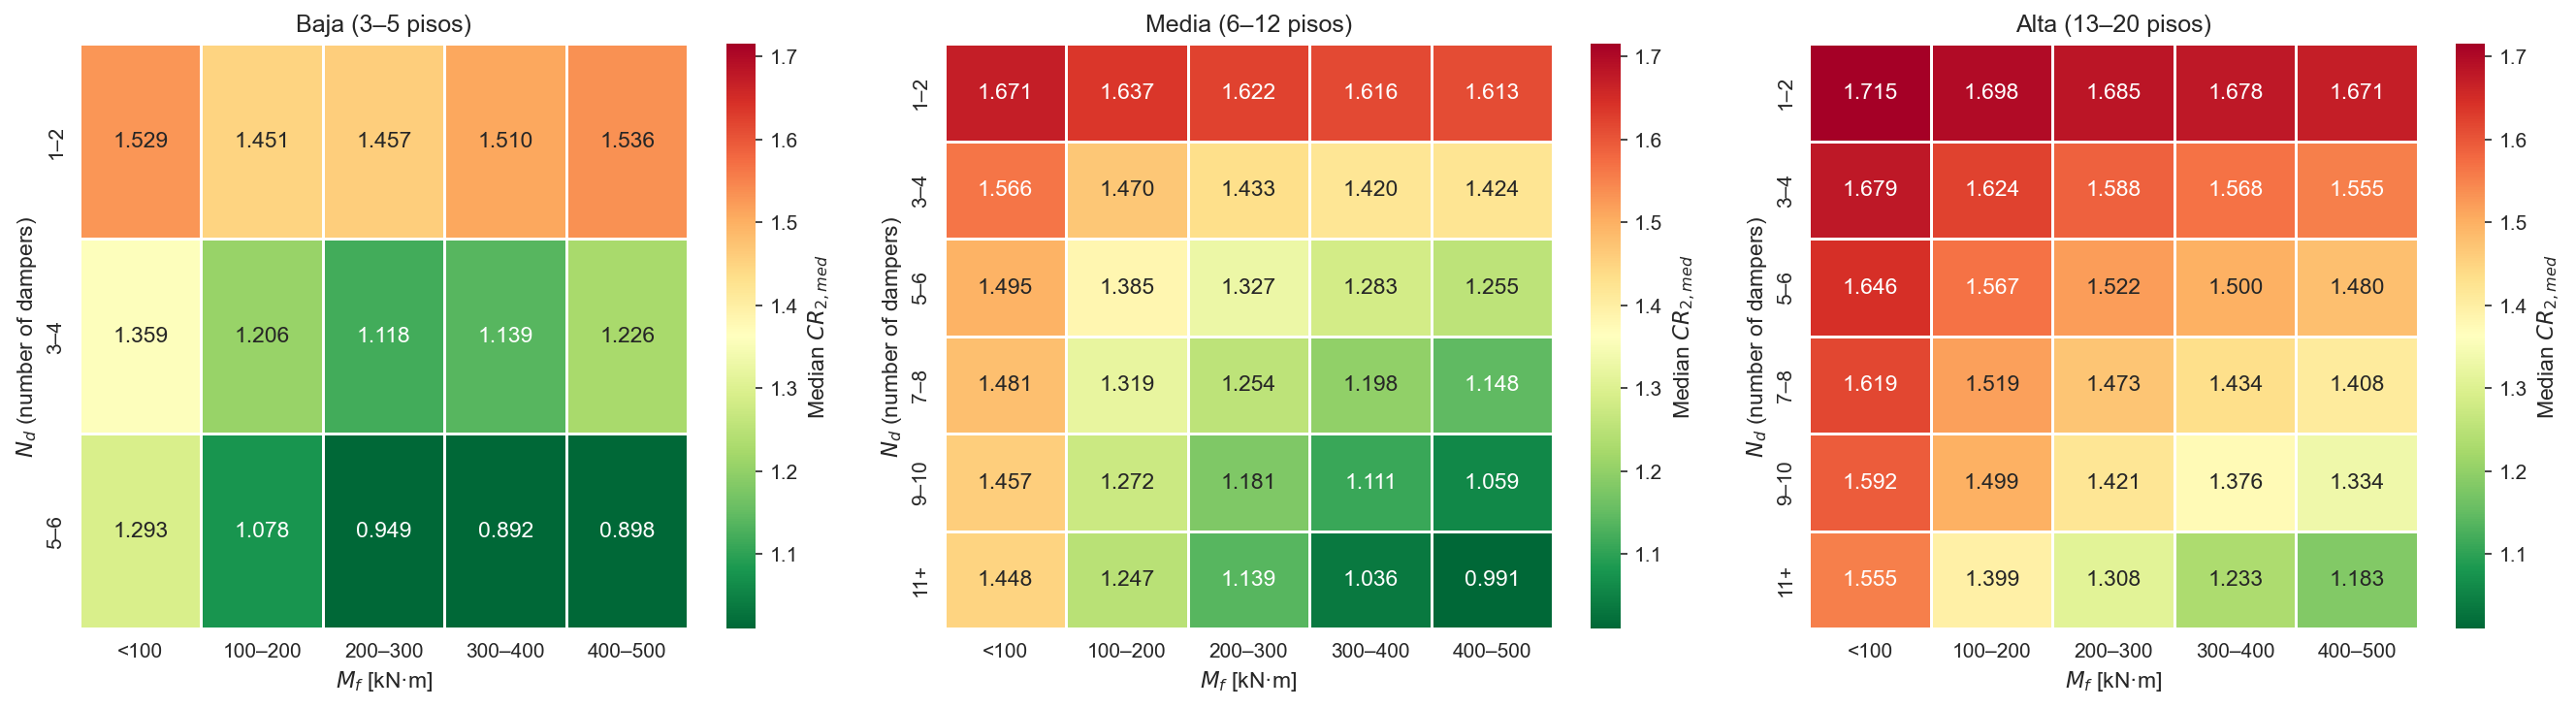
\includegraphics[width=\linewidth]{figs/F7_interaction_heatmap.png}
\caption{Izquierda: $CR_2$ mediano como función de bins de $\nd$ y bins de $\Mf$ (kN$\cdot$m), 
promediado a través de todas las estructuras y registros. Derecha: $\nd$ óptimo vs.\ $\Mf$ 
para la mejor configuración de cada estructura (color: $\CR{med}$ alcanzado).}
\label{fig:mapa_calor}
\end{figure}

\subsection{Convergencia de Diseño entre Escenarios Sísmicos}
\label{sec:results:convergencia}

La Figura~\ref{fig:convergencia} examina si un diseño óptimo único de AFR es robusto entre 
los tres escenarios sísmicos. Para cada una de las 1\,000 estructuras, se comparó el $\nd$ 
óptimo predicho bajo cada variable objetivo. La distribución de $\nd$ recomendado es 
consistente entre escenarios: mediana y P10 producen recomendaciones casi idénticas en la 
mayoría de las estructuras. El escenario P90 tiende a recomendar $\nd$ ligeramente más alto 
para edificios más altos, pero la discrepancia absoluta 
$|\nd^{\mathrm{P90}} - \nd^{\mathrm{med}}|$ se mantiene por debajo de 2 para más del 80\% 
de las estructuras. Esto significa que un diseño optimizado para el escenario mediano 
proporciona protección casi óptima a través de toda la variabilidad sísmica capturada por 
el conjunto de ocho registros.

\begin{figure}[htbp]
\centering
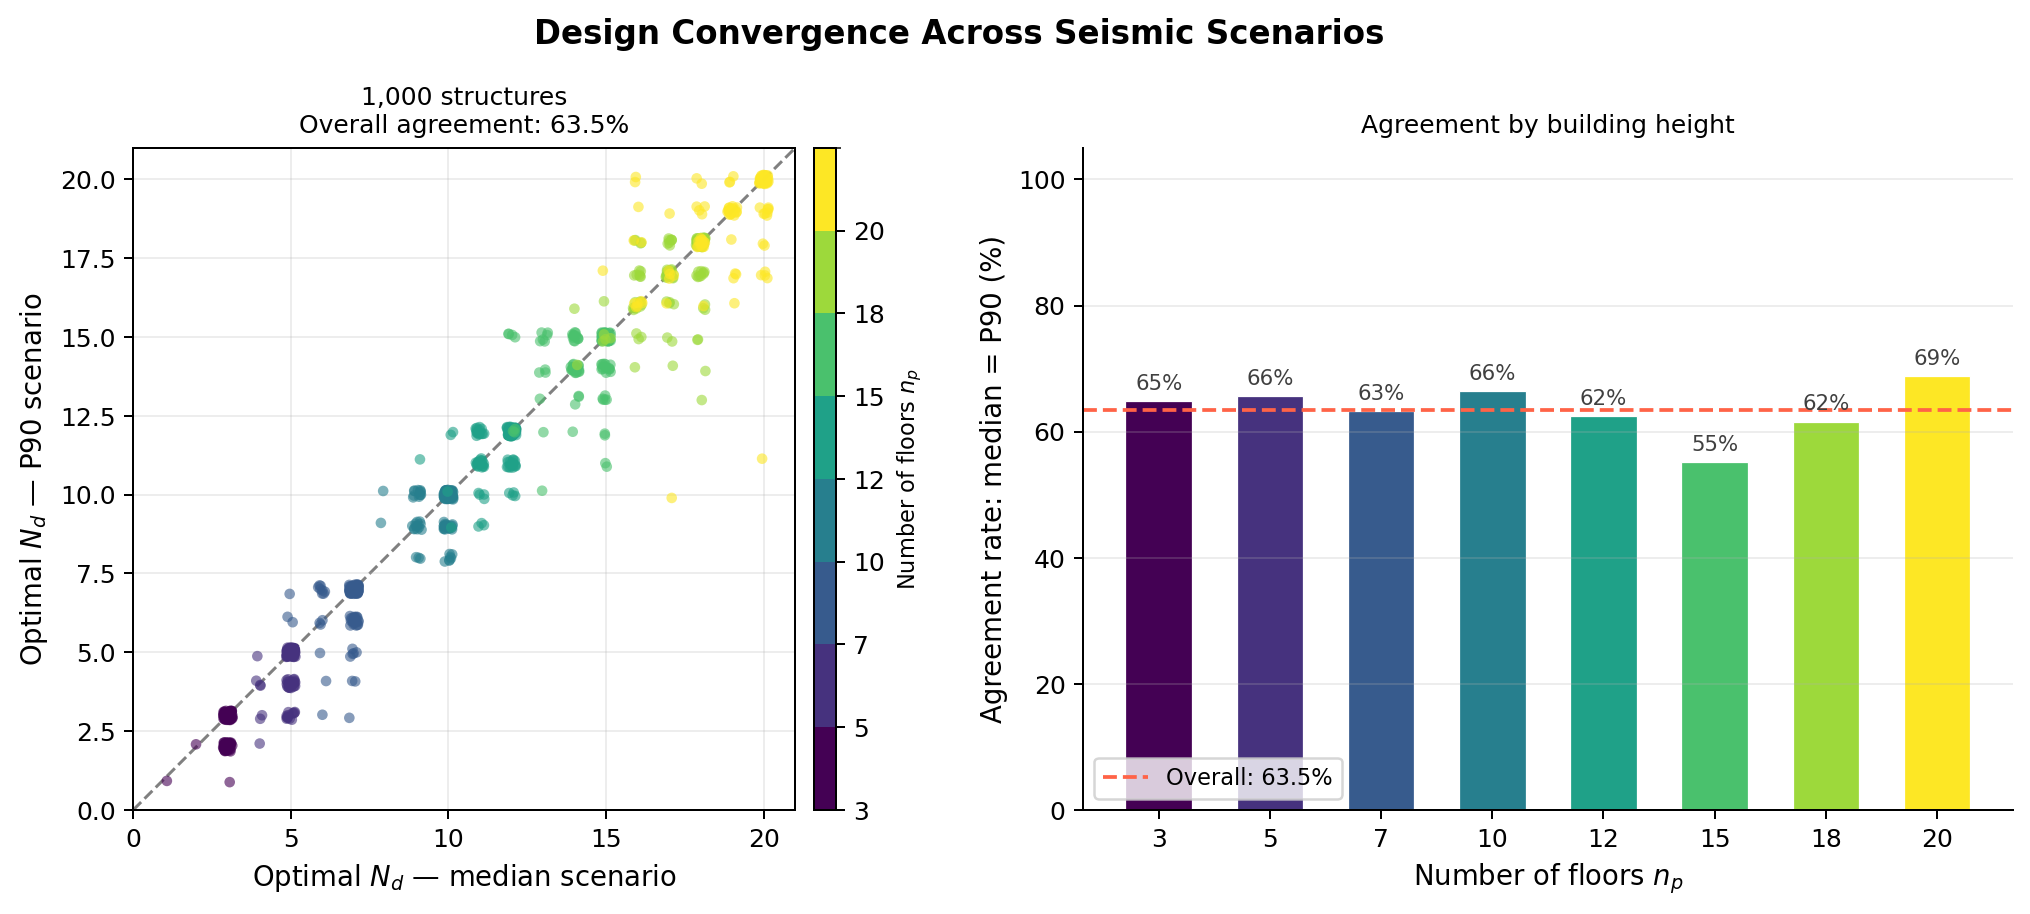
\includegraphics[width=\linewidth]{figs/F8_convergence_extended.png}
\caption{Izquierda: distribución de $\nd$ recomendado por escenario sísmico a través de las 
1\,000 estructuras. Derecha: tasa de acuerdo y discrepancia absoluta media 
$|\nd^{\mathrm{P90}} - \nd^{\mathrm{med}}|$ por altura de edificio $\np$.}
\label{fig:convergencia}
\end{figure}

%%═══════════════════════════════════════════════════════════════════════════
\section{Discusión}
\label{sec:discussion}
%%═══════════════════════════════════════════════════════════════════════════

\subsection{Densidad como Parámetro de Diseño Gobernante}

La densidad de cobertura $\etad$ es el predictor dominante de $CR_2$ ($r = -0{,}73$). El 
análisis de dominancia estocástica confirma que esta jerarquía se mantiene a través de los 
ocho registros sísmicos, independiente de otras variables de diseño 
(Sección~\ref{sec:results:decreciente}). Del análisis del umbral del 80\% de ganancia máxima, 
se sigue la siguiente recomendación de diseño: $\etad \geq 0{,}85$ para marcos de mediana y
gran altura (6--20 pisos), y $\etad \geq 0{,}95$ para marcos de baja altura (3--5 pisos),
donde cada dispositivo adicional tiene un impacto proporcionalmente mayor.

\subsection{Interacción entre Momento Friccional y Cobertura}

El análisis del mapa de calor (Figura~\ref{fig:mapa_calor}) revela una relación de sustitución 
entre $\nd$ y $\Mf$ a cobertura intermedia: duplicar $\Mf$ con un conteo fijo de dispositivos 
produce reducciones de $CR_2$ similares a agregar dos pisos de cobertura. Esta interacción no 
es capturada por correlación marginal y motiva el uso de modelos ML de ensemble que representan 
interacciones de características no lineales explícitamente. A alta cobertura 
($\etad \geq 0{,}75$), el desempeño se vuelve relativamente insensible al valor específico de 
$\Mf$ dentro de [200,\,500]\KM. El rango óptimo identificado por ML, $\Mf \in [300,\,460]$\KM,
es consistente con el rango $[81,\,439]$\KM reportado por \citet{Jarrahi2020sdee} (Tabla~3)
para un MARM de 10~pisos con seis amortiguadores bajo cinco registros sísmicos.

\subsection{Robustez entre Escenarios}

El fuerte acuerdo entre las recomendaciones de diseño medianas y P90 
(Figura~\ref{fig:convergencia}) significa que no se necesita resolver problemas de optimización 
separados para diferentes niveles de peligro cuando el objetivo es identificar el $\nd$ óptimo. 
El enfoque multi-registro aborda directamente la limitación de estudios de registro único 
\citep{Jarrahi2020jbe,Jarrahi2020sdee}, capturando variabilidad registro-a-registro a través 
de estadísticos P10, mediana y P90. Las recomendaciones ML son por tanto robustas a 
incertidumbre en la selección de acelerogramas.

\subsection{Limitaciones}

Se deben reconocer las siguientes limitaciones. (i)~Los modelos estructurales son marcos 
cortantes elásticos idealizados; la interacción no lineal marco--AFR no es capturada 
explícitamente. Los resultados son aplicables a niveles de demanda sísmica donde la respuesta 
del marco permanece elástica o cuasielástica; para sismos de alta intensidad con plastificación 
significativa del marco se esperan desviaciones respecto a las recomendaciones aquí derivadas. 
(ii)~Los ocho acelerogramas, aunque sísmicamente diversos, pueden no representar todos los 
entornos tectónicos relevantes. (iii)~La validación del modelo se basa únicamente en validación 
cruzada; un conjunto de prueba independiente proporcionaría una evaluación de generalización 
más rigurosa. (iv)~Se asume un valor uniforme de $\Mf$ por estructura; las distribuciones de 
$\Mf$ específicas por piso pueden ser preferibles en la práctica. (v)~No se incorpora función 
de costo, por lo que la optimización económica de la fracción de cobertura no se aborda.

%%═══════════════════════════════════════════════════════════════════════════
\section{Conclusiones}
\label{sec:conclusions}
%%═══════════════════════════════════════════════════════════════════════════

Las siguientes conclusiones se derivan del análisis de $\approx$434\,000 simulaciones 
tiempo-historia no lineales sobre 1\,000 configuraciones estructurales diversas y ocho 
registros sísmicos reales:

\begin{enumerate}

\item \textbf{Precisión del modelo sustituto ML.}
XGBoost y Random Forest alcanzaron $\Rsq$ de 0{,}92--0{,}93 para $\CR{med}$ y $\CR{P10}$, 
y 0{,}84 para $\CR{P90}$. Los modelos de ensemble redujeron el error de predicción en 
aproximadamente 49\% relativo a baselines lineales, cuantificando la estructura no lineal 
de la relación diseño--desempeño.

\item \textbf{La densidad de amortiguadores es la variable de diseño primaria.}
La fracción de cobertura $\etad = \nd/\np$ es el predictor más influyente ($r = -0{,}73$), 
superando sustancialmente al conteo absoluto de amortiguadores ($r = -0{,}45$). Las guías 
de diseño para AFRs deben expresarse en términos de $\etad$, no $\nd$.

\item \textbf{Umbral de rendimientos decrecientes: $\etad \approx 0{,}85$.}
El análisis intra-estructura muestra que el 80\% de la reducción máxima de $CR_2$ se alcanza
en $\etad \approx 0{,}85$ para marcos de mediana y gran altura (6--20~pisos) y en
$\etad \approx 0{,}95$ para marcos de baja altura (3--5~pisos). Estos umbrales proveen
criterios prácticos de costo-efectividad para el despliegue de AFR. El rango óptimo de
$\Mf \in [300,\,460]$\KM (mediana 400\KM) es secundario: para $\etad \geq 0{,}75$,
$CR_2$ es relativamente insensible al valor específico de $\Mf$ dentro de [200,\,500]\KM.

\item \textbf{Robustez entre escenarios.}
El $\nd$ óptimo recomendado por escenarios de mediana y P90 difiere en menos de 2 pisos en 
80\% de las estructuras analizadas. Un diseño optimizado para el escenario mediano proporciona 
protección casi óptima a través de toda la variabilidad sísmica en el conjunto de ocho registros.

\item \textbf{Trabajo futuro.}
Las extensiones deben incorporar comportamiento inelástico del marco, distribuciones de $\Mf$ 
específicas por piso, restricciones de costo de instalación, y suites de registros sísmicos 
más amplias cubriendo diferentes entornos tectónicos. La validación experimental para 
configuraciones multi-piso y la integración de modelos entrenados en una herramienta de diseño 
interactiva son direcciones inmediatas de investigación.

\end{enumerate}

%%═══════════════════════════════════════════════════════════════════════════
\section*{CRediT Author Contribution Statement}

\textbf{E.~Ponce}: Conceptualization, Methodology, Software, Formal Analysis,
Investigation, Validation, Data Curation, Visualization, Writing -- Original Draft.
\textbf{H.~Yañez-Godoy}: Conceptualization, Supervision, Writing -- Review \& Editing.

\section*{Declaration of Competing Interests}

The authors declare that they have no known competing financial interests or
personal relationships that could have appeared to influence the work reported
in this paper.

\section*{Funding}

This research did not receive any specific grant from funding agencies in the
public, commercial, or not-for-profit sectors.

\section*{Acknowledgements}

The first author gratefully acknowledges the financial support provided by the
Secretaría de Ciencias, Humanidades, Tecnología e Innovación (SECIHTI, Mexico)
through a master's scholarship. The authors also acknowledge the institutional
support of the Universidad Autónoma de Querétaro (UAQ, Mexico) and the Institut
de Mécanique et d'Ingénierie (I2M, UMR CNRS 5295), University of Bordeaux,
France.

\section*{Declaration of Generative AI and AI-Assisted Technologies in the
Writing Process}

During the preparation of this work the authors used Claude (Anthropic) in order
to assist with translation from Spanish to English and language style correction.
After using this tool, the authors reviewed and edited the content as needed and
take full responsibility for the content of the publication.

%%═══════════════════════════════════════════════════════════════════════════
\bibliographystyle{elsarticle-harv}
\bibliography{references}

\end{document}
